% CREATED BY MAGNUS GUSTAVER, 2020
\chapter{Results}\label{results}

This chapter presents the results of the project. Primarily the result corresponding to the main aim of the project, meaning the bike's ability to balance, will be presented. The results correlating to the sub-goals: how the bike performs with regards to the steering motor, forward motor and balancing algorithm are also presented. Finally the reasons behind the results, and the effects of them are discussed.

\section{Steering Motor}

The steering motor, when viewed as a standalone component fully works as intended. That is, it is disabled until the \textit{GO} button is pressed in LabVIEW, and then it can be controlled by changing the duty cycle between 10\% and 90\%. It also stops when the duty cycle is set to 50\% as expected. When the emergency stop is pressed either physically or in the software, the duty cycle is set to 50\%, and the pin is disabled. 

When connecting the control of the steering motor to the balancing algorithm and safety limit, the motor turns towards the same direction which the bike is leaning, and the duty cycle is set to 50\% when the safety limits is reached. However, the steering wheel has the possibility of overshooting the safety limit, this is caused by the inertia of the steering wheel and handlebar, it also depends on how fast it was rotating before the limit was reached.

The controls for the motors, separated into two boxes are depicted in figure \ref{fig:motorControl} below. Inside of the left box, the steering motor controls are located. In these controls there exist inputs for changing each of the PID gains labeled P, I, and D. The box also has a field for changing the angle limit (in degrees from when the wheel is straight). Below the controls mentioned above are outputs from the steering motor encoder which shows its current position, velocity and acceleration. For the purpose of calibrating the encoder, there exists a button which resets the encoder position whenever it is pressed. At the bottom of the box, the duty cycle sent to the motor from the balancing algorithm is shown. At the bottom right of the image, under the boxes, is the \textit{GO} button which starts the two motors.

\begin{figure}[ht]
    \centering
    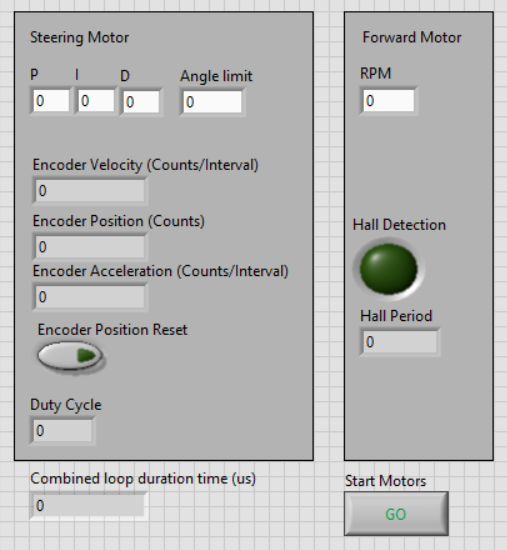
\includegraphics[width=7cm]{figure/motor_control.png}
    \caption{The motor controls in LabVIEW, with the steering motor control on the left side}
    \label{fig:motorControl}
\end{figure}

\section{Forward Motor}

The RPM of the forward motor can successfully be set using the LabVIEW front panel as seen on the right side of figure \ref{fig:motorControl} above, and also changed while the program is running. The forward motor only starts when \textit{GO} is pressed, and it stops when the emergency stop is pressed; note that this is the same behavior as the steering motor has. 

The motor can not only be controlled by setting its RPM, but also by changing its current. Controlling the motor using current can be accomplished if the function called by the \textit{Call Library Function Node} is changed to \texttt{setCurrent}. Additional methods of controlling the motor can be added by creating and calling additional C functions based on the example by Vedder.

\section{Balancing Algorithm} \label{results:balancing}

During the initial testing of the balancing algorithm, it was concluded that the steering motor behaved as expected in terms of rotation direction in relation to the roll rate of the bike. Meaning when the bike was leaned, the front wheel rotated towards the same direction. 

When the bike was then placed on the roller, it seemed as if the bike could stay upright for some time before it had to be caught to prevent it from falling. The algorithm would make the front wheel rotate to the correct direction, but the amplitude of these rotations was gradually increasing until the border of the roller was reached. A real, conclusive result could not be made from this test; the reasons for this are both because of human interference, as well as the narrow width of the roller.

The final and most reliable test of the balancing algorithm was done outdoors as described in \ref{method:unaidedTest}. The data from these tests, recorded with the logging system, are presented in the images below.

Almost all of the tests resulted in the bike falling and having to be caught within the first few seconds after being let go. The data from one such example is shown in the figures below. In figure \ref{fig:test6_control} it can be seen that the bike starts to roll left around 21.5 seconds, which leads to the duty cycle going below 50\%. The steering wheel also turns to the left around the same time, which is the expected behavior. The roll rate then increases as the bike leans to the right, and the behavior reverses.

\begin{figure}[H]
    \begin{subfigure}{.5\textwidth}
        \centering
        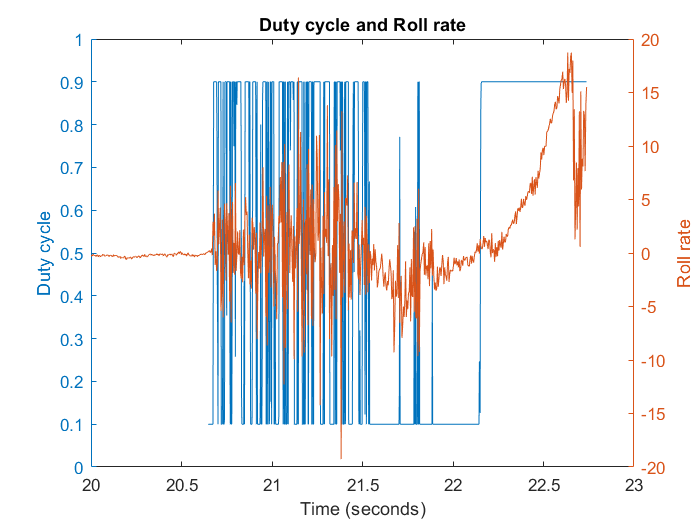
\includegraphics[width=\textwidth]{include/test6_control.png}
        \caption{The roll rate of the bike and duty cycle sent from the balancing algorithm.}
        \label{fig:test6_control}
    \end{subfigure}
    \begin{subfigure}{.5\textwidth}
        \centering
        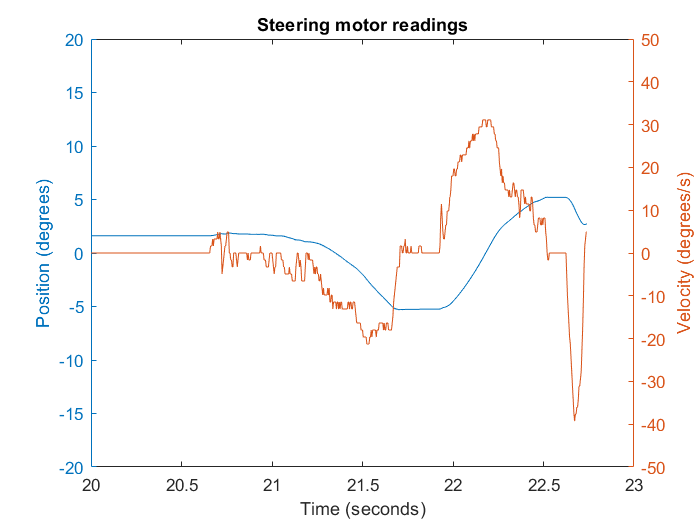
\includegraphics[width=\textwidth]{include/test6_motor.png}
        \caption{The position and velocity of steering motor.}
        \label{fig:test6_motor}
    \end{subfigure}
\caption{Plotted data from a test where the bike fell within two seconds.}
\label{fig:test6}
\end{figure}

Only a small amount of tests had the bike balancing and not falling within the first few seconds. One of these tests where the bike managed to stay upright for a longer period of time is plotted in the figures below.

\begin{figure}[H]
    \begin{subfigure}{.5\textwidth}
        \centering
        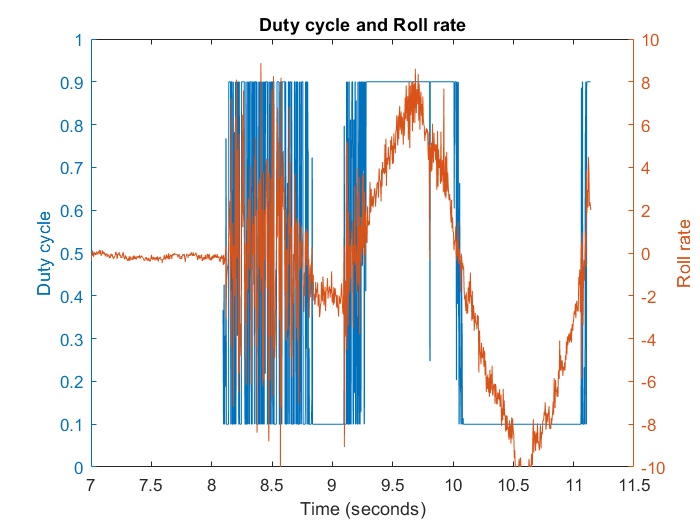
\includegraphics[width=\textwidth]{include/test4_control.png}
        \caption{The roll rate of the bike and duty cycle sent from the balancing algorithm.}
        \label{fig:test4_control}
    \end{subfigure}
    \begin{subfigure}{.5\textwidth}
        \centering
        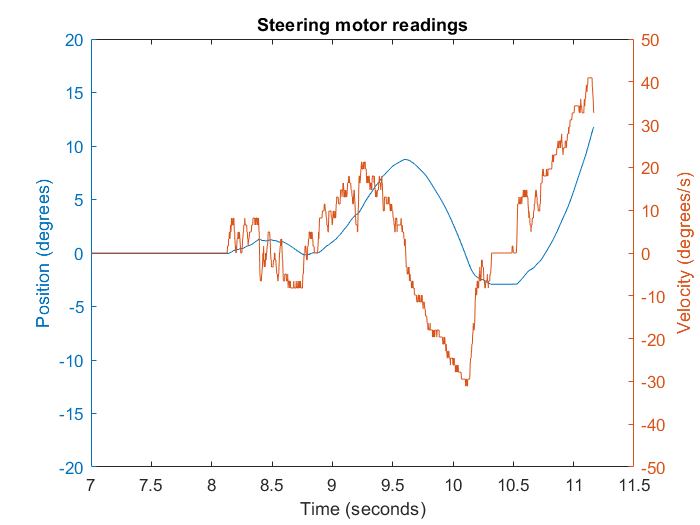
\includegraphics[width=\textwidth]{include/test4_motor.png}
        \caption{The position and velocity of steering motor.}
        \label{fig:test4_motor}
    \end{subfigure}
\caption{Plotted data from a test where the bike was driving upright for a longer distance}
\label{fig:test4}
\end{figure}

In both of the tests presented above, as well as in tests which have not been included in this report, there is a period of about 1 second between when the bike starts to drive, and when it starts to lean. This is partially caused by the bike still being held while it is reaching the set speed. During this period the roll rate fluctuates between positive and negative values with a high frequency, which also causes the duty cycle to do the same (with values above and below 50\%). This behavior is likely to be caused by vibrations in the IMU which are amplified during the acceleration. It should be noted that the duty cycle does change with a high enough frequency for the steering motor to not have enough time to start to rotate.

\section{Loop Times}

For the loop time tests all of the bikes hardware was enabled so that all control signal calculations would be made, and the resulting time would be as accurate possible. The total loop time was recorded as being between \SI{2155}{\micro\second} and \SI{2420}{\micro\second}. Compared to the previous project group's measurements, the new loop times are at worst is \SI{240}{\micro\second} slower than the worst case before the logging system and C algorithms were added \cite{AronssonKarlsson2022PROJECTAUTOBIKE}.

\section{Discussion}

The improvement of the development experience is one aim which was presented in \ref{intro:aim}, this aim is however not mentioned above. The reason being this decision it that it is difficult to assess if the aim has been reached or not, since it can be considered individual to a certain degree. What can be said is that all of the code which is used has been moved to a single location, which should make it easier to find the code. It should also now be much clearer what code is the most recent one. The code itself has been organized and separated into sub-VIs which should also make it easier to find the relevant code, this in combination with more comments should also make it easier to understand it.

When examining the plots made from the data acquired during the tests of the balancing algorithm, it is hard to draw any clear conclusions about why the bike behaves as it does. The reason for this is the limited time which the data is actually being collected. What can be extracted from the graphs is that the duty cycle reaches its limits of 0.9 and 0.1 as soon as the roll rate goes above and below 0, respectively. After examining the code in the balancing algorithm, it seems as if the most important reason behind this is the \texttt{calculateSteeringPWM} function. This function converts the angular velocity calculated by the \texttt{pid} function to the duty cycle. The function causes a small roll rate (over 0.94 when $K_p$ is 1) to result in a duty cycle outside of the allowed range. Even if the duty cycle reaches the limit when the roll rate is small, it does not seem as if the motor rotates quickly enough to stop the bike from falling.

The quick changes in roll rate caused by vibrations in the IMU is possibly due to it not being mounted properly. It is now held in place mainly by friction, which might cause it to move slightly. This is also the case for other piece of hardware used by on the bike; the battery does for example not have any sort of mounting at all, which causes it to move around as the bike leans.

The dimensions and weight of the box containing the hardware of the bike have been a concern during the entire project; not only by the project members, but also other people giving occasional help. The box is unnecessarily big which makes it heavy, it is also placed in such a way that make the center of mass be located high up from the ground. This will cause the bike to be harder to balance. The hardware inside of the box is also not placed to make their weight evenly distributed, causing the bike to more likely turn a certain direction.